\chapter{Dataset and Data Preprocessing}\label{chap:datapreprocessing}

In this chapter, we will analyze the dataset in detail, focusing on its structure, the various features it contains, and the procedures we have adopted to transform it into a new database with a better and more efficient format to be used in model training and evaluation. We will also see how the Open-Meteo meteorological service was used and how the most important features were selected to enable the training of various models.

%In questo capitolo analizzeremo nel dettaglio il dataset a nostra disposizione soffermandoci sulla sua struttura, le varie feature contnute al suo interno, e le varie procedure che abbiamo adottato per poterlo trasformare in una nuova base di dati con un formato migliore e più efficiente per essere impiegata nell'addestramento e valutazione dei modelli. Vedremo anche come è stato utilizzato il servizio meteorologico OpenMeteo e soprattutto come sono state poi selezionate le feature più importanti per rendre possibile l'addestramento dei vari modelli.

\section{Dataset} \label{sec:dataset}

The dataset at our disposal describes a period of almost two years
(from 02-02-2022 to 16-06-2023) and comes from a 978 kW photovoltaic
plant located in the province of Bari. It consists of 3 inverters,
27 field panels, 1 meter, 1 solarimeter, 2 interface protections
and 1 \textquote{system} device in which data from Solargis are stored.
The dataset is organized into files, one for each type of device,
representing each individual day, and the data is aggregated
every 5 minutes. Each row contains a reference to the device
it belongs to (\verb|deviceName| and \verb|deviceId|).


%Il dataset a nostra disposizione descrive un periodo di quasi due anni (dal
%02/02/2022 al 16/06/2023) ed è proveniente da un impianto fotovoltaico da 978 kW
%situato nella provincia di Bari. È composto da
%3 inverter, 27 quadri di campo, 1 contatore, 1 solarimetro, 2 protezioni
%interfaccia e 1 dispositivo \textquote{impianto} nel quale vengono immagazzinati
%i dati provenienti da Solargis. Il dataset è organizzato in file, uno per
%tipologia di dispositivo, che
%rappresentano la singola giornata e i dati sono aggregati a 5 minuti ed ogni
%riga riporta il riferimento al
%dispositivo di appartenenza (\verb|deviceName| e \verb|deviceId|).

\begin{table}[H]
	\begin{center}
		\begin{tabular}[c]{l}
			\hline
			\textbf{File Name}                                  \\
			\hline
			\verb|2022_02_02_Rofilo_NP00003174_inverter.csv|    \\
			\verb|2022_02_02_Rofilo_NP00003174_meteorology.csv| \\
			\verb|2022_02_02_Rofilo_NP00003174_meter.csv|       \\
			\verb|2022_02_02_Rofilo_NP00003174_other.csv|       \\
			\verb|2022_02_02_Rofilo_NP00003174_plantDevice.csv| \\
			\verb|2022_02_02_Rofilo_NP00003174_stringbox.csv|   \\
			\verb|2022_02_03_Rofilo_NP00003174_inverter.csv|    \\
			\verb|2022_02_03_Rofilo_NP00003174_meteorology.csv| \\
			\verb|2022_02_03_Rofilo_NP00003174_meter.csv|       \\
			\verb|2022_02_03_Rofilo_NP00003174_other.csv|       \\
			\verb|2022_02_03_Rofilo_NP00003174_plantDevice.csv| \\
			\verb|2022_02_03_Rofilo_NP00003174_stringbox.csv|   \\
			$\ldots$                                            \\
			\hline
		\end{tabular}
	\end{center}
	\caption{Some files from our dataset.}\label{tab:datasunto}
\end{table}

\begin{table}[H]
	\begin{center}
		\begin{tabular}[c]{l|l|l|l|l|l}
			\hline
			\multicolumn{1}{c|}{\textbf{timestamp}}        &
			\multicolumn{1}{c|}{\textbf{serial}}           &
			\multicolumn{1}{c|}{\textbf{$\ldots$}}         &
			\multicolumn{1}{c|}{\textbf{TotalEnergy(kWh)}} &
			\multicolumn{1}{c|}{\textbf{Frequency(Hz)}}    &
			\multicolumn{1}{c}{\textbf{deviceid}}            \\
			\hline
			2022-10-23 04:30:00                            &
			INV01                                          &
			$\ldots$                                       &
			357196.88                                      &
			50.06                                          &
			83204                                            \\

			2022-10-23 04:35:00                            &
			INV01                                          &
			$\ldots$                                       &
			357196.88                                      &
			50.06                                          &
			83204                                            \\

			%			01/02/2023 00:15                               &
			%			INV01                                          &
			%			$\ldots$                                       &
			%			431324.36                                      &
			%			49.88                                          &
			%			83204                                            \\

			$\ldots$                                       &
			$\ldots$                                       &
			$\ldots$                                       &
			$\ldots$                                       &
			$\ldots$                                       &
			$\ldots$                                         \\
			2022-10-23 13:00:00                            &
			INV01                                          &
			$\ldots$                                       &
			357921.16                                      &
			49.95                                          &
			83204                                            \\
			2022-10-23 13:05:00                            &
			INV01                                          &
			$\ldots$                                       &
			357935.24                                      &
			49.95                                          &
			83204                                            \\
			%			01/02/2023 12:10                               &
			%			INV01                                          &
			%			$\ldots$                                       &
			%			431324.36                                      &
			%			49.88                                          &
			%			83204                                            \\

			$\ldots$                                       &
			$\ldots$                                       &
			$\ldots$                                       &
			$\ldots$                                       &
			$\ldots$                                       &
			$\ldots$                                         \\
			01/02/2023 23:45                               &
			INV01                                          &
			$\ldots$                                       &
			431324.36                                      &
			49.88                                          &
			83204                                            \\
			01/02/2023 23:50                               &
			INV01                                          &
			$\ldots$                                       &
			431324.36                                      &
			49.88                                          &
			83204                                            \\
			%			01/02/2023 23:55                               &
			%			INV01                                          &
			%			$\ldots$                                       &
			%			431324.36                                      &
			%			49.88                                          &
			%			83204                                            \\
			\hline
		\end{tabular}
		\caption{Some lines from an Inverter file.}\label{tab:invsunto}
	\end{center}
\end{table}

\subsection{Inverter}
Inside the files related to the inverters, we can find data such as
the processor's operating temperature
(\verb|InternalTemperature|), various Alternating and Direct currents
produced (\verb|CurrentAC| and \verb|CurrentDC|), Delivered Power,
total energy produced by the individual inverter and other status
and control bits that indicate various stages of the inverter's
life (boot, reset, ready, etc.).

Down below a table with all the available features:


%Nei file relativi agli inverter posiamo trovare dati come la temperatura di
%funzionamento del processore (\verb|InternalTemperature|), le varie correnti
%alternate e continue prodotte (\verb|CurrentAC| e \verb|CurrentDC|), la Potenza Erogata, l'energia totale prodotta dal singolo inverter più altri
%bit di stato e controllo che mostrano le varie fasi di vita dell'inverter (boot, reset, ready, ecc.).\\
%Di seguito una tabella con tutte le features a disposizione:
%Un inverter in un impianto fotovoltaico è un componente fondamentale che svolge
%una funzione vitale: converte l'energia elettrica prodotta dai pannelli solari,
%che è in corrente continua (DC), in energia elettrica utilizzabile in corrente
%alternata (AC). Questa conversione è cruciale perché la maggior parte delle
%apparecchiature elettriche domestiche e delle reti di distribuzione elettrica
%utilizzano corrente alternata per funzionare.
%Regolano la
%tensione e la frequenza della corrente alternata prodotta per garantire che
%siano conformi agli standard di rete elettrica locale. Questo è importante
%per evitare danni agli apparecchi elettrici e per garantire
%l'interoperabilità con la rete elettrica.
%Sono spesso dotati di
%tecnologie avanzate come il "Maximum Power Point Tracking" (MPPT) che
%ottimizzano costantemente la produzione di energia solare. Questo significa
%che l'inverter regola la tensione in ingresso dai pannelli solari per
%ottenere la massima potenza possibile in base alle condizioni di luce solare
%in tempo reale.
%Le feature che caratterizzano il nostro impianto sono riassunte dalla seguente
%tabella:

\begin{table}[H]
	\begin{center}
		\begin{tabular}[c]{l|l|l}
			\hline
			\multicolumn{1}{c|}{\textbf{Name}}        &
			\multicolumn{1}{c|}{\textbf{Unit Symbol}} &
			\multicolumn{1}{c}{\textbf{Description}}                                     \\
			\hline
			CommunicationCode                         & -   & Communication Code         \\
			Failure 3                                 & -   & Active Alarm               \\
			Failure 4                                 & -   & Isolation Alarm            \\
			CurrentDC                                 & A   & Photovoltaic field Current \\
			CurrentAC                                 & A   & Network Current            \\
			CurrentAC Phase1                          & A   & Line RMS Current Phase R   \\
			CurrentAC Phase2                          & A   & Line RMS Current Phase S   \\
			CurrentAC Phase3                          & A   & Line RMS Current Phase T   \\
			TotalEnergy                               & kWh & Active Energy Delivered    \\
			Frequency                                 & Hz  & Network Frequency          \\
			PowerAC Phase1                            & kW  & Line PA Phase R            \\
			PowerAC Phase2                            & kW  & Line PA Phase S            \\
			PowerAC Phase3                            & kW  & Line PA Phase T            \\
			PowerAC                                   & kW  & Delivered PA               \\
			PowerDC                                   & kW  & Photovoltaic field Power   \\
			Status                                    & -   & Inverter State             \\
			Failure                                   & -   & Network docking PLL State  \\
			Failure 2                                 & -   & Network State 1            \\
			Failure 1                                 & -   & Network State  2           \\
			InternalTemperature                       & C   & CPU Temp.                  \\
			HeatSinkTemperature                       & C   & IGBT Temp.                 \\
			VoltageDC                                 & V   & Photovoltaic field Voltage \\
			VoltageAC                                 & V   & Network Voltage            \\
			VoltageAC Phase1                          & V   & Line RMS Voltage Phase R   \\
			VoltageAC Phase2                          & V   & Line RMS Voltage Phase S   \\
			VoltageAC Phase3                          & V   & Line RMS Voltage Phase T   \\
			\hline
		\end{tabular}
		\caption{All available features from an \texttt{inverter} file.}\label{tab:invfeatures}
	\end{center}
\end{table}

\begin{figure}[H]
	\centering
	\begin{subfigure}[t]{0.45\textwidth}
		\centering
		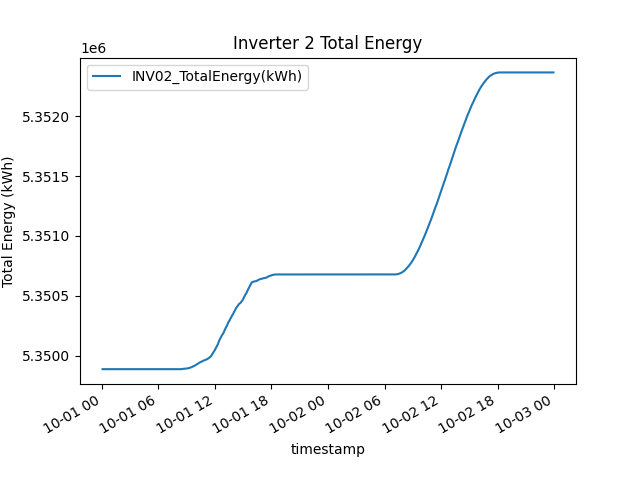
\includegraphics[width=\textwidth, keepaspectratio]{chapters/1_introduction/imgs/inv2totenergy.png}
		\caption{Inverter 2 Total Energy plot.}
		\label{fig:inv02totenergy}
	\end{subfigure}
	\hspace{0.5cm}
	\begin{subfigure}[t]{0.45\textwidth}
		\centering
		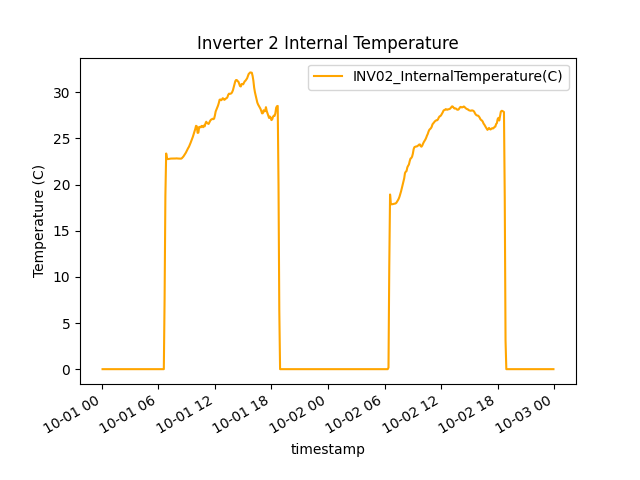
\includegraphics[width=\textwidth, keepaspectratio]{chapters/1_introduction/imgs/inv2temperature.png}
		\caption{Inverter 2 CPU Temperature plot.}
		\label{fig:inv02temp}
	\end{subfigure}\\

	\begin{subfigure}[t]{0.45\textwidth}
		\centering
		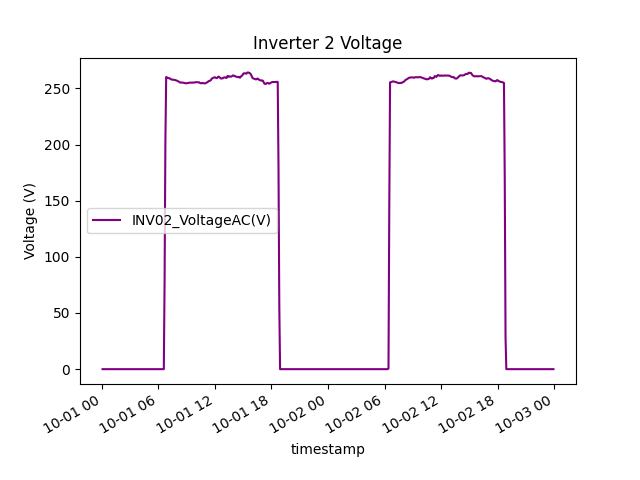
\includegraphics[width=\textwidth, keepaspectratio]{chapters/1_introduction/imgs/inv2voltage.png}
		\caption{Inverter 2 Voltage AC plot.}
		\label{fig:inv02volt}
	\end{subfigure}
	\hspace{0.5cm}
	\begin{subfigure}[t]{0.45\textwidth}
		\centering
		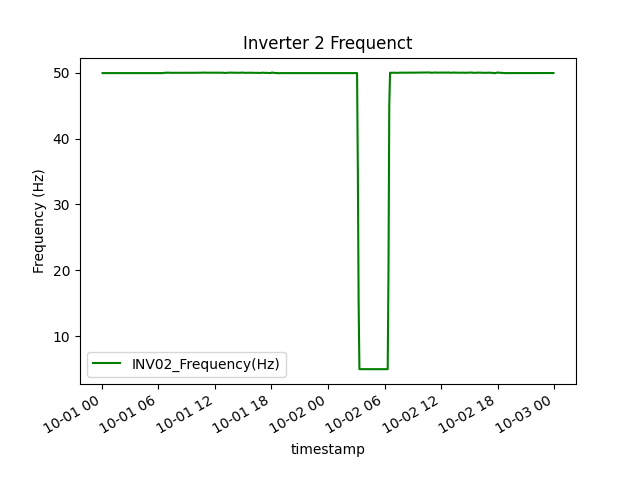
\includegraphics[width=\textwidth, keepaspectratio]{chapters/1_introduction/imgs/inv2freq.png}
		\caption{Inverter 2 Frequency plot.}
		\label{fig:inv02freq}
	\end{subfigure}
\end{figure}


%\subsection{StringBox}
%Le stringbox in un impianto fotovoltaico sono contenitori elettrici progettati
%per ospitare e proteggere una serie (o stringa) di pannelli solari collegati in
%serie. Questi dispositivi svolgono diverse funzioni importanti:
%
%\begin{itemize}
%	\item Protezione: Le stringbox includono dispositivi di protezione come interruttori
%	      automatici o fusibili che prevengono cortocircuiti e sovraccarichi nel circuito
%	      fotovoltaico.
%	\item Connettori: Forniscono connettori sicuri per collegare i cavi provenienti dai
%	      pannelli solari alla stringa di cavi principale dell'impianto.
%	\item Monitoraggio: Alcune stringbox sono dotate di sistemi di monitoraggio che
%	      consentono di rilevare prestazioni o guasti dei pannelli solari all'interno
%	      della stringa.
%	\item Isolamento: Possono anche includere dispositivi di isolamento che consentono di
%	      interrompere l'alimentazione elettrica verso la stringa di pannelli solari per
%	      scopi di manutenzione o sicurezza.
%\end{itemize}

\subsection{Junction Box}
In the files related to the Junction Box or Combiner Box, we find data that describes
the current production of the various strings they are connected to (\verb|CurrentString1-7|,
in general, each Junction Box manages 7 strings), some temperatures (such as
\verb|ModuleTemperature|), and some control bits to check proper operation.


%Nei file relativi alle Junction Box o Combiner Box, troviamo dati che
%descrivono la produzione di corrente delle varie stringhe a cui sono collegati (\verb|CurrentString1-7|, in generale ogni Junction Box gestisce 7 stringhe), alcune temperature (come \verb|ModuleTemerature|) e alcuni bit di controllo per verificare il corretto funzionamento.

\begin{table}[H]
	\begin{center}
		\begin{tabular}[c]{l|l|l}
			\hline
			\multicolumn{1}{c|}{\textbf{Name}}        &
			\multicolumn{1}{c|}{\textbf{Unit Symbol}} &
			\multicolumn{1}{c}{\textbf{Description}}                                             \\
			\hline
			CommunicationCode                         & -              & Communication Code      \\
			Failure                                   & -              & Strings Alarm           \\
			CurrentString1                            & A              & Current I1              \\
			CurrentString2                            & A              & Current I2              \\
			CurrentString3                            & A              & Current I3              \\
			CurrentString4                            & A              & Current  I4             \\
			CurrentString5                            & A              & Current I5              \\
			CurrentString6                            & A              & Current I6              \\
			CurrentString7                            & A              & Current I7              \\
			AverageStringCurrent                      & A              & Average Current         \\
			Irradiance                                & $\text{W/m}^2$ & Modules Irradiation     \\
			Failure 1                                 & -              & Open Strings            \\
			Failure 2                                 & -              & Not Perform. Strings    \\
			EnvironmentTemperature                    & C              & Environment Temperature \\
			ModuleTemperature                         & C              & Modules Temperature     \\
			InternalTemperature                       & C              & Board Temperature       \\
			\hline
		\end{tabular}
		\caption{All available features form a \texttt{stringbox} file.}\label{tab:junctionfeatures}
	\end{center}
\end{table}


\subsection{Solargis} \label{sec:solargis}
Solargis is a company specialized in providing solar data and forecasting services for photovoltaic
installations and solar energy-related projects. Their main goal is to provide precise and
reliable information on solar irradiation and solar weather conditions anywhere in the world.
This data is essential for the design, optimization, and management of photovoltaic systems.
Solargis collects and provides detailed data on global, direct, and diffuse solar irradiation at
every geographical location. This data allows photovoltaic system developers to assess the
amount of available solar energy in a given area, which is crucial for properly sizing the
system and calculating production forecasts.

%Solargis è una società specializzata nella fornitura di dati e servizi di
%previsione solare per impianti fotovoltaici e progetti legati all'energia
%solare. Il loro principale obiettivo è fornire informazioni precise e affidabili
%sull'irradiazione solare e sulle condizioni meteorologiche solari in qualsiasi
%parte del mondo. Questi dati sono fondamentali per la progettazione,
%l'ottimizzazione e la gestione degli impianti fotovoltaici.
%Solargis raccoglie e fornisce dati dettagliati
%sull'irradiazione solare globale, diretta e diffusa in ogni posizione
%geografica. Questi dati consentono agli sviluppatori di impianti fotovoltaici di
%valutare la quantità di energia solare disponibile in una determinata area, il
%che è fondamentale per dimensionare correttamente l'impianto e calcolare le
%previsioni di produzione.

\begin{table}[H]
	\begin{center}
		\begin{tabular}[c]{l|l|l|l}
			\hline
			\multicolumn{1}{c|}{\textbf{timestamp}}         &
			\multicolumn{1}{c|}{\textbf{$\ldots$}}          &
			\multicolumn{1}{c|}{\textbf{SolargisGHI(W/m2)}} &
			\multicolumn{1}{c}{\textbf{SolargisGTI(W/m2)}}                          \\
			\hline
			2022-08-01 11:40:00                             & $\ldots$ & 896 & 978  \\
			2022-08-01 11:45:00                             & $\ldots$ & 896 & 978  \\
			2022-08-01 11:50:00                             & $\ldots$ & 896 & 978  \\
			2022-08-01 11:55:00                             & $\ldots$ & 914 & 1001 \\
			2022-08-01 12:00:00                             & $\ldots$ & 914 & 1001 \\
			2022-08-01 12:05:00                             & $\ldots$ & 914 & 1001 \\
			2022-08-01 12:10:00                             & $\ldots$ & 928 & 1019 \\
			2022-08-01 12:15:00                             & $\ldots$ & 928 & 1019 \\
			2022-08-01 12:20:00                             & $\ldots$ & 928 & 1019 \\

			\hline
		\end{tabular}
		\caption{Some Solargis data from \texttt{2022\_08\_01\_Rofilo\_NP00003174\_plantDevice.csv} file}\label{tab:solargis}
	\end{center}
\end{table}

\begin{figure}[H]
	\centering
	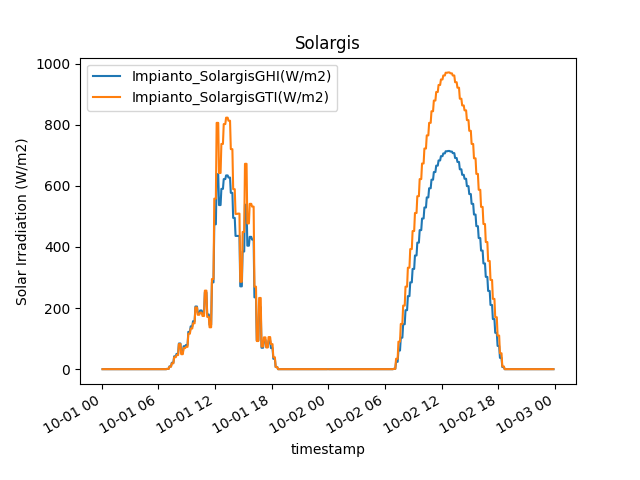
\includegraphics[width=.7\linewidth]{chapters/1_introduction/imgs/solargis.png}
	\caption{Solargis GHI \& GTI plot.}
	\label{fig:solargisplot}
\end{figure}


Solar radiation takes a long journey until it reaches Earth’s surface. So when
modelling solar radiation, various interactions of extra-terrestrial solar
radiation with the Earth’s atmosphere, surface and objects are to be taken into
account. The component that is neither reflected nor scattered, and which
directly
reaches the surface, is called direct radiation; this is the component that
produces shadows. The component that is scattered by the atmosphere, and which
reaches the ground is called diffuse radiation. The small part of the radiation
reflected by the surface and reaching an inclined plane is called the reflected
radiation. These three components together create global radiation.

In solar energy applications, the following parameters are commonly used in
practice:

\begin{itemize}
	\item Direct Normal Irradiation/Irradiance (DNI) is the component that is
	      involved in thermal (concentrating solar power, CSP) and photovoltaic
	      concentration
	      technology (concentrated photovoltaic, CPV).
	\item  Global Horizontal
	      Irradiation/Irradiance (GHI) is the sum of direct and diffuse radiation
	      received on a horizontal plane. GHI is a reference radiation for the
	      comparison of climatic zones; it is also essential parameter for
	      calculation of radiation on a tilted plane.
	\item Global Tilted Irradiation/Irradiance (GTI), or total
	      radiation received on a surface with defined tilt and azimuth, fixed or
	      sun-tracking. This is the sum of the scattered radiation, direct and
	      reflected. It is a reference for photovoltaic (PV) applications, and
	      can be occasionally affected by shadow.
\end{itemize}


\begin{table}[H]
	\begin{center}
		\begin{tabular}[c]{l|l|l}
			\hline
			\multicolumn{1}{c|}{\textbf{Name}}        &
			\multicolumn{1}{c|}{\textbf{Unit Symbol}} &
			\multicolumn{1}{c}{\textbf{Description}}                                                            \\
			\hline
			SolargisGHI                               & $\text{W/m}^2$ & Solargis Global Horizontal Irradiation \\
			SolargisGTI                               & $\text{W/m}^2$ & Solargis Global Tilted Irradiation     \\
			\hline
		\end{tabular}
		\caption{All available features from a \texttt{plantDevice} file.}\label{tab:solargisfeatures}
	\end{center}
\end{table}

\subsection{Meteorology}
In the Meteo files, we can find some environment
temperature and solar irradiance data. Is important to mention that these
features are not as powerful as
weather forecast or Solargis data for the Imputation task.

%Nei file meteo possiamo trovare alcuni dati sulla temperatura
%ambientale e il valore dell'irraggiamento solare. Non risultano
%dati completi come potrebbero essere quelli provenienti da
%previsioni meteo.

\begin{table}[H]
	\begin{center}
		\begin{tabular}[c]{l|l|l}
			\hline
			\multicolumn{1}{c|}{\textbf{Name}}        &
			\multicolumn{1}{c|}{\textbf{Unit Symbol}} &
			\multicolumn{1}{c}{\textbf{Description}}                                        \\
			\hline
			COMMUNICATION\_CODE SOL                   & -              & Communication Code \\
			Irradiance SOL                            & $\text{W/m}^2$ & Irradiance         \\
			Module Temperature HEX SOL                & -              & All Registers      \\
			Module Temperature SOL                    & C              & Module Temperature \\
			\hline
		\end{tabular}
		\caption{All available features from a \texttt{meteo} file.}\label{tab:solargisfeatures}
	\end{center}
\end{table}

\subsection{Meter}
The Meter files contain information about the current injected
into and drawn from the network. It is from here that we get
the values of our target feature \verb|Cont_TotalEnergy(kWh)|.

%I file meter contengono informazioni sulla corrente immessa e prelevata dalla rete.
%\`{E} da qui che andremo a leggere i valori della nostra target feature \verb|Cont_TotalEnergy(kWh)|.

\begin{figure}[H]
	\centering
	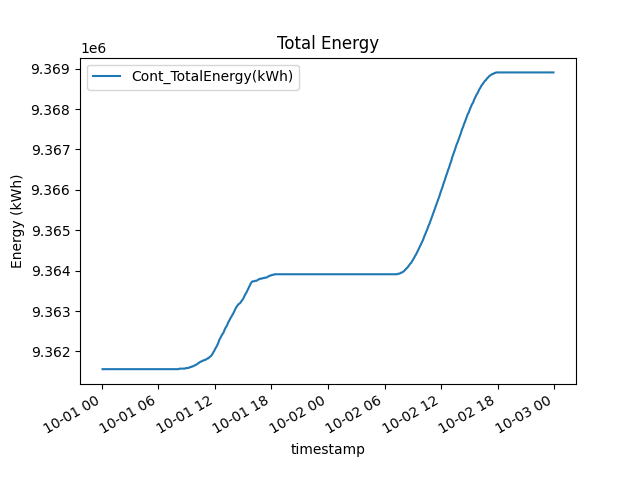
\includegraphics[width=1\linewidth]{chapters/1_introduction/imgs/totalenergy.png}
	\caption{Total Energy plot, our target feature.}
	\label{fig:totenergyplot}
\end{figure}

\begin{table}[H]
	\begin{center}
		\begin{tabular}[c]{l|l|l}
			\hline
			\multicolumn{1}{c|}{\textbf{Name}}        &
			\multicolumn{1}{c|}{\textbf{Unit Symbol}} &
			\multicolumn{1}{c}{\textbf{Description}}                                \\
			\hline
			COMMUNICATION\_CODE Cont                  & -   & Communication Code    \\
			Status Cont                               & -   & Status                \\
			Totale Energia Immessa Cont               & kWh & Total Energy          \\
			Totale Energia Prelevata Cont             & kWh & Total Energy Imported \\
			\hline
		\end{tabular}
		\caption{All available features from a \texttt{meter} file.}\label{tab:meterfeatures}
	\end{center}
\end{table}

\subsection{Other}
In the Other type files, we can find the remaining,
less relevant, features
that describe the behavior and functioning of the leftover elements
that make up the photovoltaic plant system.

%Nei file di tipo other possiamo trovare altre feature meno rilevanti che vanno
%a descrivere il comportamento e il funzionmento degli altri elementi che compongono
%l'impiato solare.

\begin{table}[H]
	\begin{center}
		\begin{tabular}[c]{l|l|l}
			\hline
			\multicolumn{1}{c|}{\textbf{Name}}        &
			\multicolumn{1}{c|}{\textbf{Unit Symbol}} &
			\multicolumn{1}{c}{\textbf{Description}}                            \\
			\hline
			COMMUNICATION\_CODE NV10P                 & -  & Communication Code \\
			CB-State NV10P                            & -  & CB State           \\
			Frequency NV10P                           & Hz & Frequency          \\
			IN1 NV10P                                 & -  & Digital IN 1       \\
			IN2 NV10P                                 & -  & Digital IN 2       \\
			Last Trip Cause NV10P                     & -  & Last Trip Cause    \\
			NV10P - Trip BF                           & -  & Digital IN 25      \\
			NV10P - Trip f<                           & -  & Digital IN 24      \\
			NV10P - Trip f>                           & -  & Digital IN 23      \\
			NV10P - Trip U<                           & -  & Digital IN 21      \\
			NV10P - Trip U>                           & -  & Digital IN 22      \\
			UE NV10P                                  & V  & UE                 \\
			UL1 NV10P                                 & V  & Voltage AC Phase 1 \\
			UL2 NV10P                                 & V  & Voltage AC Phase 2 \\
			UL3 NV10P                                 & V  & Voltage AC Phase 3 \\
			Un NV10P                                  & V  & Un                 \\
			Unp NV10P                                 & V  & Unp                \\
			COMMUNICATION\_CODE NA16                  & -  & Communication Code \\
			CB-State NA16                             & -  & CB State           \\
			IE NA16                                   & A  & IE                 \\
			IL1 NA16                                  & A  & Current AC Phase 1 \\
			IL2 NA16                                  & A  & Current AC Phase 2 \\
			IL3 NA16                                  & A  & Current AC Phase 3 \\
			IN1 NA16                                  & -  & Digital IN 1       \\
			IN2 NA16                                  & -  & Digital IN 2       \\
			NA16 - Protection Trip                    & -  & Digital IN 25      \\
			\hline
		\end{tabular}
		\caption{All available features from an \texttt{other} file.}\label{tab:otherfeatures}
	\end{center}
\end{table}

%Avere il dataset suddiviso in diversi file, uno per giorno e per
dispositivo (vedi Sezione \ref{sec:dataset}), con la presneza di
alcuni periodi, che vanno da pochi minuti a diversi gionri, di assenza dati
(dovuti probabilmente ad un fallimento dello strumento di raccolta dati)
fa sì che si verifichino molti problemi durante la fase di training
e la rende quasi impossibile. In questo capitolo vedremo come abbiamo
risolto questi problemi, optando per una struttura tabellare monolitica
del dataset e quali approccia abbiamo utilizzato per la gestione
dei dati mancanti.
\section{Dataset Realization}
%{\bf (*VP* se sposti la sez 1.7, devi distinguere fra il dataset dei dati originali e quello ottenuto dalla loro lavorazione. Il primo potrebbe essere "Original Dataset"}

For the creation of a dataset taht can be passed directly to our imputation models, we devised a procedure that
allowed us to merge all the original files into a single file, where for
each timestamp, we have all the data for the entire system at
that exact moment. Below is the final structure of the dataset
and the algorithm for generating it.

%Per la realizzazione del nostro dataset abbiamo ideato 
%una procedura che ci ha permesso di ottenere un unico file,
%in formato csv, dove, per ogni time stamp abbiamo tutti i dati
%di tutto l'impianto in quell'esatto istante. Di seguito 
%la struttira finale del dataset e l'algoritmo per generarlo.


\begin{table}[H]
	\begin{center}
		\begin{tabular}[c]{l|l|l|l}
			%\hline
			\multicolumn{1}{c|}{\textbf{timestamp}}              &
			\multicolumn{1}{c|}{\textbf{DEV.NAME$_1$\_FEAT$_1$}} &
			\multicolumn{1}{c|}{$\ldots$}                        &
			\multicolumn{1}{c}{\textbf{DEV.NAME$_n$\_FEAT$_n$}}                                   \\
			\hline

			01/10/2022 10:00                                     & $\ldots$ & $\ldots$ & $\ldots$ \\
			01/10/2022 10:05                                     & $\ldots$ & $\ldots$ & $\ldots$ \\
			01/10/2022 10:10                                     & $\ldots$ & $\ldots$ & $\ldots$ \\
			%\hline
		\end{tabular}
	\end{center}
	\caption{Final dataset feature structure.}\label{tab:datasetform}
\end{table}

\begin{algorithm}[H]
	\caption{Dataset aggregation algorithm}\label{alg:dataset}
	\begin{algorithmic}
		\Require data\_folder
		\Ensure \texttt{data\_folder} exists
		\State dev\_types $\gets$ find all file types inside \texttt{data\_folder} (e.g. meter, inverter, $\ldots$)
		\State dev\_content $\gets$ a dictionary with \texttt{dev\_types} types as $keys$ and empty $values$

		\For {\textbf{each} key \textbf{in} dev\_conent.keys}
		\State files $\gets$ find all file matching type \texttt{key} inside \texttt{data\_folder}
		\State sort \texttt{files} by date (asc.)
		\State temp\_type\_aggregate $\gets$ and empty csv table
		\For {\textbf{each} file \textbf{in} files}
		\State append all \texttt{file} lines to \texttt{temp\_type\_aggregate} table
		\EndFor
		\State dev\_content[key] $\gets$ temp\_type\_aggregate
		\EndFor
		\State\Comment{At this time we have a dictionary mapping a file type with all its available data}
		\State
		\State dataset $\gets$ an empty csv table
		\For {\textbf{each} type, data \textbf{in} dev\_content} \Comment{\texttt{type} is $key$, \texttt{data} is $value$}
		\State rename all \texttt{data} $columns$ to \texttt{data.deviceID}\_\texttt{$column$.name}
		\State except for 'timestamp' $column$
		\State dataset $\gets$ \texttt{dataset} and \texttt{data} tables using 'timestamp' column
		\EndFor
		\State save \texttt{dataset} table to file
	\end{algorithmic}
\end{algorithm}

\begin{table}[H]
	\begin{center}
		\begin{tabular}[c]{l|l|l|l}
			%\hline
			\multicolumn{1}{c|}{\textbf{timestamp}}      &
			\multicolumn{1}{c|}{\textbf{INV01\_PowerAC}} &
			\multicolumn{1}{c|}{\textbf{$\ldots$}}       &
			\multicolumn{1}{c}{\textbf{Cont\_TotalEnergy}}                                 \\
			\hline
			2022-02-02 00:05:00                          & NaN      & $\ldots$ & NaN       \\
			2022-02-02 00:10:00                          & NaN      & $\ldots$ & NaN       \\
			$\ldots$                                     & $\ldots$ & $\ldots$ & $\ldots$  \\
			2022-06-22 10:20:00                          & 175.66   & $\ldots$ & 8900941.5 \\
			2022-06-22 10:25:00                          & 178.29   & $\ldots$ & 8900995.5 \\
			2022-06-22 10:30:00                          & 180.82   & $\ldots$ & 8901036.0 \\
			$\ldots$                                     & $\ldots$ & $\ldots$ & $\ldots$  \\
			2023-06-16 18:00:00                          & NaN      & $\ldots$ & NaN       \\
			2023-06-16 18:05:00                          & NaN      & $\ldots$ & NaN       \\
		\end{tabular}
	\end{center}
	\caption{Some data from dataset after running Algorithm~\ref{alg:dataset}}\label{tab:datasetfinalvalues}
\end{table}

\subsection{Timestamp cyclical encoding}
To enable the models to learn the alternation of minutes, days,
and months as effectively as possible during the training phase,
we applied a procedure to transform each individual timestamp into
a pair of sine and cosine values, thus performing a cyclic
encoding of various seasonalities.

%Per permettere ai modelli, durante la fase di allenamento, di apprendere
%al meglio possibile l'alternarsi dei minuti, giorni e mesi abbiamo
%applicato una procedura per trasfrormare ogni signolo timestamp
%in una coppia di valori seno-coseno effettuando così un 
%encoding ciclico delle varie stagionalità.


\begin{algorithm}[H]
	\caption{Cyclical Encoding Algorithm}\label{alg:cyclicencoding}
	\begin{algorithmic}
		\Require dataset table
		\Ensure \texttt{dataset} \textbf{is not} empty
		\State dataset['minute\_sin'] $\gets \sin(2 \pi (\frac{\text{\texttt{dataset.timestamp.minute}}}{60}))$
		\State dataset['minute\_cos'] $\gets \cos(2 \pi (\frac{\text{\texttt{dataset.timestamp.minute}}}{60}))$


		\State dataset['hour\_sin'] $\gets \sin(2 \pi (\frac{\text{\texttt{dataset.timestamp.hour}}}{24}))$
		\State dataset['hour\_cos'] $\gets \cos(2 \pi (\frac{\text{\texttt{dataset.timestamp.hour}}}{24}))$


		\State dataset['day\_sin'] $\gets \sin(2 \pi (\frac{\text{\texttt{dataset.timestamp.day}}}{31}))$
		\State dataset['day\_cos'] $\gets \cos(2 \pi (\frac{\text{\texttt{dataset.timestamp.day}}}{31}))$

		\State dataset['month\_sin'] $\gets \sin(2 \pi (\frac{\text{\texttt{dataset.timestamp.month}}}{12}))$
		\State dataset['month\_cos'] $\gets \cos(2 \pi (\frac{\text{\texttt{dataset.timestamp.month}}}{12}))$
	\end{algorithmic}
\end{algorithm}

\begin{figure}[H]
	\centering
	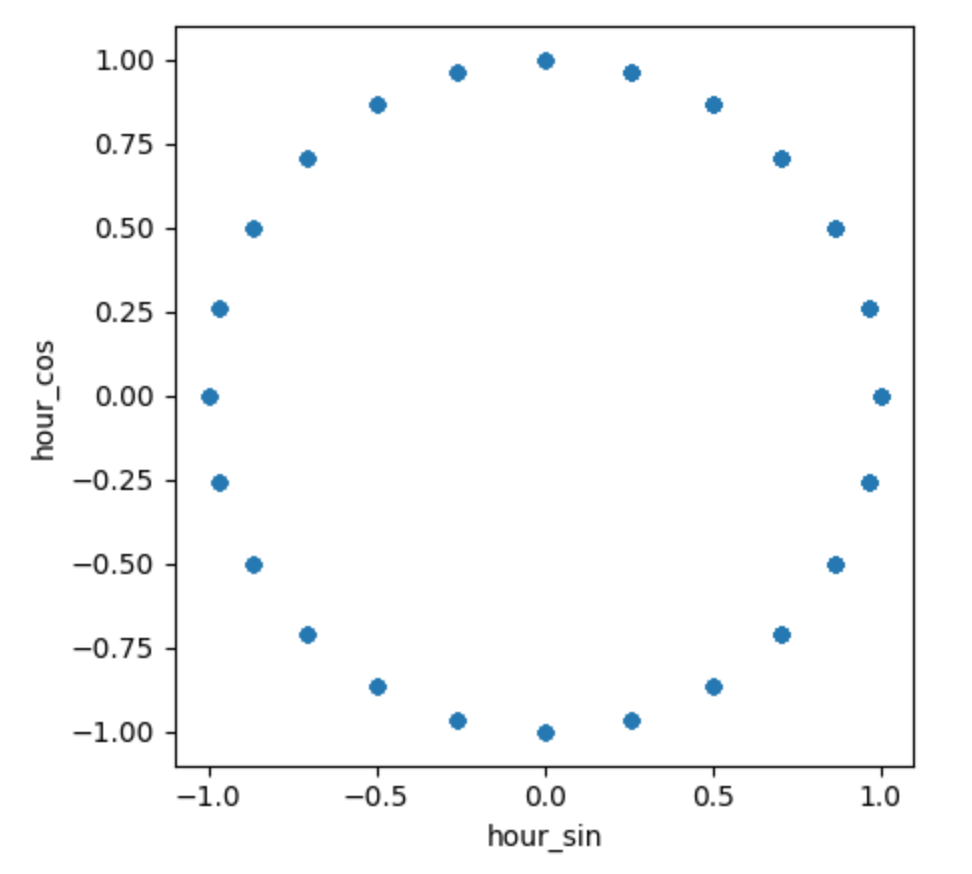
\includegraphics[width=0.7\linewidth, keepaspectratio]{chapters/2_data_preprocessing/imgs/hoursincosplot.png}
	\caption{Hour cyclical encoding plot.}\label{fig:encodingplot}
\end{figure}

\subsection{Historical weather}
In addition to the information from Solargis (see Section~\ref{sec:solargis}),
the models may require other weather data, such as cloud cover, rainfall, etc.
Therefore, we made an API call to Open-Meteo servers (see Section~\ref{sec:openmeteo}), using the \textquote{Historical Weather} functionality, to obtain the accurate past
forecasts for the time period covered by our dataset (from 02-02-2022 to 18-06-2023).

%Oltre alle infomazioni provenienti da Solargis
%(vedi Sezione \ref{sec:solargis}), i modelli potrebbero avere bisogno
%di altri dati meteo, come la presenza di nuvole, pioggia, ecc.
%Abbiamo quindi effettuato una chiamata API ai server di Open-Meteo (vedi
%Sezione \ref{sec:openmeteo}), usando la funzionalità
%\textquote{Historical Weather}, per ottenere le previsioni passate
%esatte del periodo temporale che copre il nostro dataset (dal 02-02-2022 al 18-06-2023).

\begin{algorithm}[H]
	\caption{Open-Meteo data request Algorithm}\label{alg:openemeteo}
	\begin{algorithmic}
		\Require dataset table
		\Ensure \texttt{dataset} \textbf{is not} empty

		\State meteo\_data $\gets$ require meteo feature from Open-Mete public API
		\State dataset $\gets$ merge \texttt{dataset} and \texttt{meteo\_data} tables using \texttt{timestamp} column

		\State
		\State /* At this time we have \texttt{dataset} timestamps as 5 minute frequency and \texttt{meteo\_data} as 1 hour frequency. */
		\State

		\State use a \textit{forward fill} method to fill gaps inside \texttt{dataset} table only for \texttt{meteo\_data} columns.
	\end{algorithmic}
\end{algorithm}

We have obtained most of the information made available by Open-Meteo since the API
request is free \cite{openmeteo} and computationally and storage-wise inexpensive.
These will be filtered at a later time (see Section~\ref{sec:featureselection}).
Among these, we find \texttt{sunrise} and \texttt{sunset}, which indicate the exact time
(down to the minute) of when dawn and sunset occurred, respectively.
These two features will be used to create a new column in our dataset called
\texttt{is\_day}, which will allow the model to understand whether it is
analyzing a period of time during the day or night.
This is to ensure that it does not make energy production predictions
during the night.

%Abbiamo preso la maggior parte delle informazioni messe a disposizione 
%da Open-Meteo dato che la richiesta API è gratuita e poco costosa a
%livello computazionale e di archiviazione. Queste verranno poi filtrate in un
%momento successivo (vedi Sezione \ref{sec:featureselection}).
%Tra queste troviamo \texttt{sunrise} e \texttt{sunset} che stanno
%ad indicare rispettivamente l'ora esatta (con precisione al minuto) di
%quando è avvenuta l'alba e l'ora esatta (con precisione al minuto) di
%quando è avvenuto il tramonto. Queste due feature ci serviranno per 
%costruire una nuova colonna nel nostro dataset, denominata \texttt{is\_day}, che permetterà al modello di comprendere se sta analizzando un
%periodo di tempo dove è giorno o nette. Questo per assicurarci che
%non daranno come predizioni produzioni di energia duarante la notte.

%\newpage
\begin{longtable}[c]{p{0.3\linewidth}|p{0.07\linewidth}| p{0.54\linewidth}}
	\hline
	\multicolumn{1}{c|}{\textbf{Feature}}                                                                                                                                                   &
	\multicolumn{1}{c|}{\textbf{Unit}}                                                                                                                                                      &
	\multicolumn{1}{c}{\textbf{Note}}                                                                                                                                                                                                                                                                                                                                                                                                                                                                                          \\
	\hline
	\verb|temperature_2m|                                                                                                                                                                   & °C                      & Air temperature at 2 meters above ground.                                                                                                                                                                                                                                                              \\
	\verb|relativehumidity_2m|                                                                                                                                                              & \%                      & Relative humidity at 2 meters above ground.                                                                                                                                                                                                                                                            \\
	\verb|dewpoint_2m|                                                                                                                                                                      & °C                      & Dew point temperature at 2 meters above ground. The dew point of a given body of air is the temperature to which it must be cooled to become saturated with water vapor. This temperature depends on the pressure and water content of the air.                                                        \\ %% preso da: https://en.wikipedia.org/wiki/Dew_point
	\verb|apparent_temperature|                                                                                                                                                             & °C                      & Apparent temperature is the perceived feels-like temperature combining wind chill factor, relative humidity and solar radiation.                                                                                                                                                                       \\
	\verb|precipitation|                                                                                                                                                                    & mm                      & Total precipitation (rain, showers, snow) sum of the preceding hour. Data is stored with a 0.1 mm precision. If precipitation data is summed up to monthly sums, there might be small inconsistencies with the total precipitation amount.                                                             \\
	\verb|weathercode|                                                                                                                                                                      & wmo                     & Weather condition as a numeric code. Follow WMO weather interpretation codes. Weather code is calculated from cloud cover analysis, precipitation and snowfall. As barely no information about atmospheric stability is available, estimation about thunderstorms is not possible.                     \\
	\verb|pressure_msl| \verb|surface_pressure|                                                                                                                                             & hPa                     & Atmospheric air pressure reduced to mean sea level (msl) or pressure at surface. Typically pressure on mean sea level is used in meteorology. Surface pressure gets lower with increasing elevation.                                                                                                   \\

	\verb|cloudcover| 	Instant                                                                                                                                                              & \%                      & Total cloud cover as an area fraction.                                                                                                                                                                                                                                                                 \\

	\verb|et0_fao_| \verb|evapotranspiration|                                                                                                                                               & mm                      & $ET_0$ Reference Evapotranspiration of a well watered grass field. Based on FAO-56 Penman-Monteith equations $ET_0$ is calculated from temperature, wind speed, humidity and solar radiation. Unlimited soil water is assumed. $ET_0$ is commonly used to estimate the required irrigation for plants. \\
	\verb|vapor_pressure_| \verb|deficit|                                                                                                                                                   & kPa                     & Vapor Pressure Deificit (VPD) in kilopascal (kPa). For high VPD (>1.6), water transpiration of plants increases. For low VPD (<0.4), transpiration decreases.                                                                                                                                          \\
	\verb|windspeed_10m| \verb|windspeed_100m|                                                                                                                                              & km/h                    & Wind speed at 10 or 100 meters above ground. Wind speed on 10 meters is the standard level.                                                                                                                                                                                                            \\
	\verb|winddirection_10m| \verb|winddirection_100m|                                                                                                                                      & °                       & Wind direction at 10 or 100 meters above ground.                                                                                                                                                                                                                                                       \\
	\verb|windgusts_10m |                                                                                                                                                                   & km/h                    & Gusts at 10 meters above ground of the indicated hour. Wind gusts in CERRA are defined as the maximum wind gusts of the preceding hour.                                                                                                                                                                \\ %Please consult the ECMWF IFS documentation for more information on how wind gusts are parameterized in weather models.\\
	\verb|soil_temperature_0_| \verb|   to_7cm| \verb|soil_temperature_7_| \verb|   to_28cm| \verb|soil_temperature_28_| \verb|   to_100cm| \verb|soil_temperature_100_| \verb|   to_255cm| & °C                      & Average temperature of different soil levels below ground.                                                                                                                                                                                                                                             \\
	                                                                                                                                                                                        &                         &                                                                                                                                                                                                                                                                                                        \\
	\verb|soil_moisture_0_| \verb|   to_7cm| \verb|soil_moisture_7_| \verb|   to_28cm| \verb|soil_moisture_28_| \verb|   to_100cm| \verb|soil_moisture_100_| \verb|   to_255cm|             & $\text{m}^3/\text{m}^3$ & Average soil water content as volumetric mixing ratio at 0-7, 7-28, 28-100 and 100-255 cm depths.                                                                                                                                                                                                      \\
	\caption{All feature selected from Open-Meteo with description\cite{openmeteo}.}\label{tab:openmeteofeatures}
\end{longtable}
\newpage
The new feature \texttt{is\_day} contains two values: 0 and 1,
representing \textit{Night} and \textit{Day}, respectively.
To create this feature, we add 0 with a frequency of 5 minutes until sunrise,
then add 1 until sunset, and finally add more 0s until the end of the day.
We repeat this process for each day in the dataset to create a new column that,
for each timestamp, will indicate whether it is day or night.

%La nuova feature \texttt{is\_day} conterrà due valori 0 e 1 che rappresenteranno 
%rispettivamente \textit{Notte} e \textit{Giorno}. Per la creazione di questa feature
%aggiungiamo 0, con frequenza di 5 minuit, fin all'ora dell'alba, poi degli 1 fino al
%tramonto e poi altri 0 fino alla fine del giorno. Ripetiamo questa operazione per tutti
%i giorni del dataset così da ottenere una nuova colonna che, per ogni timestamp, ci dirà se è giorno o notte.

\begin{algorithm}[H]
	\caption{is\_day feature generation Algorithm}\label{alg:isday}
	\begin{algorithmic}
		\Require dataset table, sunrise and sunset table
		\Ensure \texttt{dataset} \textbf{is not} empty, \texttt{sunrise} and \texttt{sunset} tables \textbf{match} \texttt{dataset} days

		\State is\_day $\gets$ empty table column
		\For{\textbf{each} day \textbf{in} dataset.days}
		\State temp\_is\_day $\gets$ empty table column
		\State day\_start $\gets$ sunrise[day] \Comment{get sunrise timestamp for that day}
		\State day\_start $\gets$ find the nearest \texttt{dataset.timestamp} to \texttt{day\_start}

		\State day\_end $\gets$ sunset[day]
		\State day\_end $\gets$ find the nearest \texttt{dataset.timestamp} to \texttt{day\_end}
		\State /* if \texttt{sunrise[day] = 7:04} then \texttt{day\_start = 7:05} */
		\State
		\State /* 0 means Night, 1 mean Day */
		\State temp\_is\_day $\gets$ add 0s starting from 00:00 to \texttt{day\_start}

		as 5 minute frequency
		\State temp\_is\_day $\gets$ add 1s starting from \texttt{day\_start} to \texttt{day\_end}

		as 5 minute frequency
		\State temp\_is\_day $\gets$ add 0s starting from \texttt{day\_end} day end

		as 5 minute frequency
		\State \textbf{append} to \texttt{is\_day} column \texttt{temp\_is\_day} values
		\EndFor
		\State \textbf{merge} \texttt{is\_day} column to \texttt{dataset} table
	\end{algorithmic}
\end{algorithm}

%\begin{lstlisting}[captionpos=b, caption=HTTP GET request to Open-Meteo API.]
%GET / HTTP/1.1 
%Host: archive-api.open-meteo.com/v1/archive  
%
%latitude=...&longitude=...&
%start_date=2022-02-02&
%end_date=2023-06-18&
%
%hourly=temperature_2m,relativehumidity_2m,dewpoint_2m,
%       apparent_temperature,precipitation,weathercode,
%       pressure_msl,surface_pressure,cloudcover,
%       et0_fao_evapotranspiration,
%       vapor_pressure_deficit,windspeed_10m,
%       windspeed_100m,winddirection_10m,
%       winddirection_100m,windgusts_10m,
%       soil_temperature_0_to_7cm,soil_temperature_7_to_28cm,
%       soil_temperature_28_to_100cm,
%       soil_temperature_100_to_255cm,
%       soil_moisture_0_to_7cm,soil_moisture_7_to_28cm,
%       soil_moisture_28_to_100cm,soil_moisture_100_to_255cm&
%
%daily=sunrise,sunset&
%timezone=Europe%2FBerlin
%
%\end{lstlisting}

\subsection{Dealing with gaps}

\begin{figure}[H]
	\centering
	\begin{subfigure}[t]{0.48\textwidth}
		\centering
		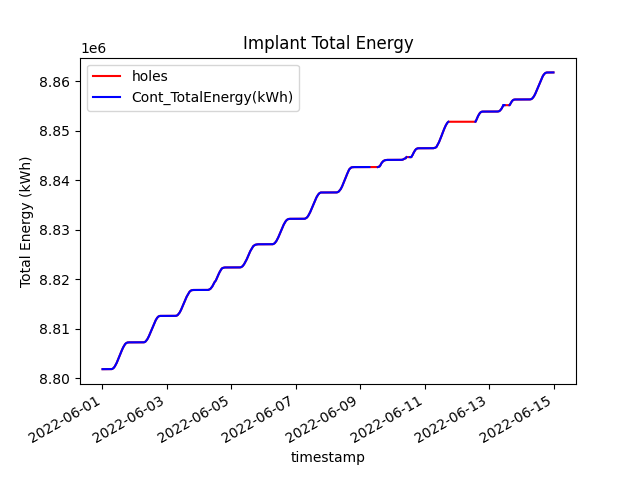
\includegraphics[width=\textwidth, keepaspectratio]{chapters/2_data_preprocessing/imgs/totenergybuco1.png}
	\end{subfigure}
	\hspace{0.1cm}
	\begin{subfigure}[t]{0.48\textwidth}
		\centering
		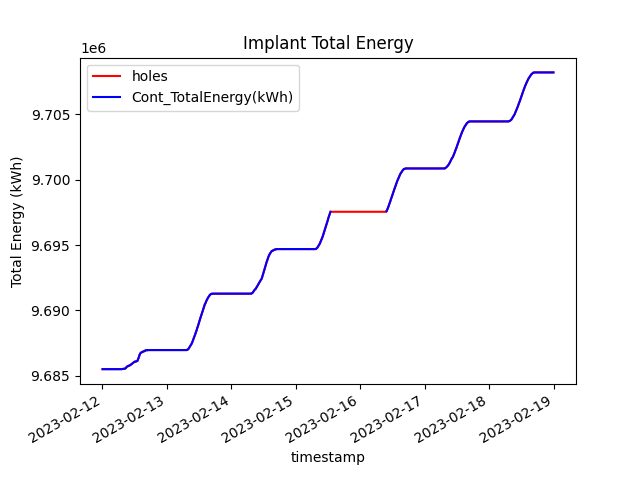
\includegraphics[width=\textwidth, keepaspectratio]{chapters/2_data_preprocessing/imgs/totenergybuco2.png}
	\end{subfigure}\\

	\begin{subfigure}[t]{0.48\textwidth}
		\centering
		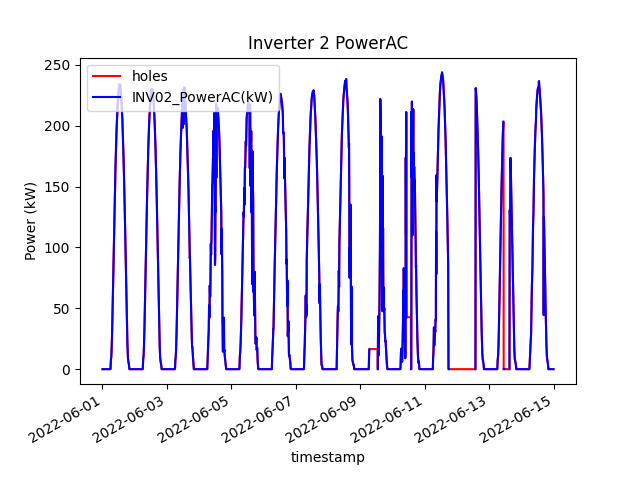
\includegraphics[width=\textwidth, keepaspectratio]{chapters/2_data_preprocessing/imgs/inv02powerbuco1.png}
	\end{subfigure}
	\hspace{0.1cm}
	\begin{subfigure}[t]{0.48\textwidth}
		\centering
		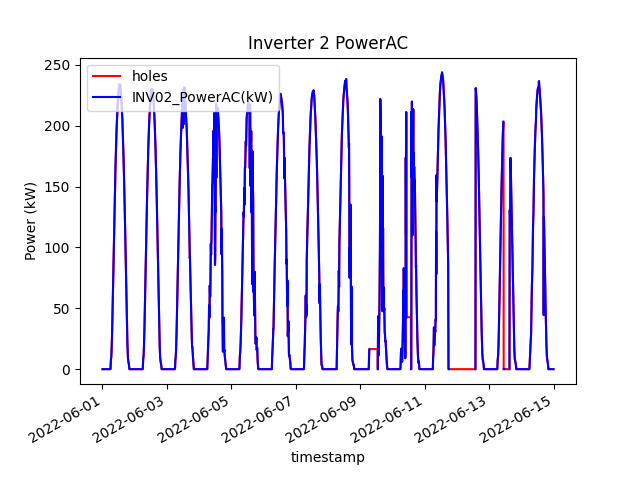
\includegraphics[width=\textwidth, keepaspectratio]{chapters/2_data_preprocessing/imgs/inv02powerbuco1.png}
	\end{subfigure}
	\caption{Some dataset \textquote{holes}. The charts at the top refer to the Implant's Total Energy, while those at the bottom refer to the Inverter 2's Power. The charts on the left range from 01-06-2022 to 15-06-2022, while those on the right range from 12-02-2023 to 19-02-2023.}\label{fig:graficibuchi}
\end{figure}

As we can see from Figure~\ref{fig:graficibuchi}, there are certain
periods within the dataset (highlighted in red) where data is missing,
which we refer to as \textquote{holes}. These data gaps can cause problems during model training
(hindering the correct calculation of the loss function), and therefore,
they need to be removed.

One possible approach for holes removal
is to perform a \textit{fill} operation: filling the gap with the
first available non-null value. This tactic may be considered
acceptable only if the time span involves just a few timestamps.
However, if we are talking about several hours or even days, it
significantly distorts the overall production and instantaneous
power trends, resulting, especially in very unfortunate cases, with extremely abnormal production curves.

The solution we have adopted to address this problem is the removal of
the entire day when a hole occurs. For example, if we have a data
gap from 12-02-2023 23:00 to 13-02-2023 10:40, the days
12-02-2023 and 13-02-2023 will be completely removed. With this
method, we lose some data, but as we will see later, the number of
gaps is not extremely high, and this data loss is not
debilitating. The following algorithm summarizes what has
just been described.

%Come possiamo vedere dalla Figura \ref{fig:graficibuchi}, all'interno del dataset sono presenti alcuni periodi (evidenziati in rosso) di assenza dati che è ciò che chiamiamo \textquote{buco}.
%Lasciare questi buchi causa problemi durante l'allenamento dei modelli (impediscono il corretto calcolo della loss function) e per questo
%vanno rimossi. Un possibile approccio per la loro rimozione è effettuare
%un'operazione di \textquote{fill}: riempio il buco con il primo valore non nullo disponibile.
%Questa tattica può essere ritenuta accettabile solo se il lasso di tempo coinvolge solo qualche timestamp, se invece parliamo di
%qualche ora o addirittura giorni questo va ad alterare notevolmente
%l'andamento della produzione totale e della potenza istantanea, risultando in casi molto sfortunati, ad avere curve di produzione estremamente anomale.
%
%La soluzione che abbiamo adottato per risolvere questo problema è
%l'eliminazione di tutto il giorno in cui si presenta il buco.
%Per fare un esempio pratico, se abbiamo un buco di dati che va dal
%12-02-2023 23:00 al 13-02-2023 10:40, verranno completamente eliminati
%i giorni 12-02-2023 e 13-02-2023. Con questo metodo andiamo a perdere 
%alcuni dati, ma come vedremo poi, il numero dei buchi non è estremamente
%elevato e la perdita di questi dati non risulta invalidante. Il seguente algoritmo riassume quanto appena detto.
%
\noindent\begin{minipage}[t]{0.55\linewidth}
	\begin{algorithm}[H]
		\caption{Holes Removal Algorithm.}\label{alg:holes}
		\begin{algorithmic}
			\Require dataset table
			\Ensure \texttt{dataset} \textbf{is not} empty

			\State holes $\gets$ find all timestamp from \texttt{dataset} table, where there are some \texttt{Nan}s inside the columns
			\For{\textbf{each} row \textbf{in} \texttt{dataset.rows}}
			\If {row.timestamp \textbf{is in} \texttt{holes}}
			\State drop \texttt{row} from \texttt{dataset} table
			\EndIf
			\EndFor
		\end{algorithmic}
	\end{algorithm}

\end{minipage}%
\hfill%
\begin{minipage}[t]{0.30\linewidth}
	\begin{table}[H]
		\centering
		\begin{tabular}[c]{l}
			\multicolumn{1}{c}{\textbf{Timestamp}} \\
			\hline
			2022-06-09                             \\
			2022-06-10                             \\
			2022-06-11                             \\
			2022-06-12                             \\
			2022-06-13                             \\
			2022-06-28                             \\
			2022-06-29                             \\
			2022-06-30                             \\
			2022-08-26                             \\
			2022-09-23                             \\
			2022-10-06                             \\
			2023-02-03                             \\
			2023-02-15                             \\
			2023-02-16                             \\
			2023-03-26                             \\
		\end{tabular}
		\caption{Timestamps deleted after running the Algorithm~\ref{alg:holes}}
	\end{table}
\end{minipage}

\subsection{Target Feature}
For the deep learning models that we will introduce later,
it could be very difficult learning how to predict the Total Missing Energy,
as it is a curve that grows constantly, potentially to infinity.
These models need to have features that vary within a limited range of
values. To achieve this, we transformed the variable
\verb|Cont_TotalEnergy(kWh)| from cumulative to instantaneous values of
produced energy, thereby limiting its values within a finite range.
This new feature was added to the dataset with the name \verb|target|.

%Per i modelli di deep learning che presenteremo successivamente, potrebbe
%risultare molto difficile imparare a prevedere l'Energia Totale mancante
%in quanto è una curva che cresce costantemente, potenzialmente all'infinito.
%Questi modelli hanno bisogno di avere features che variano in un range 
%limitato di valori. Per ottenere ciò abbiamo trasformato la variabile
%\verb|Cont_TotalEnergy(kWh)| da cumulata a valori istantanei di energia prodotta, andando così a limitare i suoi valori in un range finito. 
%Questa nuova feature è stata aggiunta al dataset con il nome di \verb|target|.

\begin{algorithm}[H]
	\caption{Cumulative Energy to Instant Energy Algorithm.}\label{alg:cumtoinstant}
	\begin{algorithmic}
		\Require dataset table
		\Ensure \texttt{dataset} \textbf{is not} empty

		\State target $\gets$ empty column
		\For{\textbf{each} (prev\_val, val) \textbf{in} dataset["Cont\_TotalEnergy(kWh)"]}
		\State diff $\gets \text{val} - \text{prev\_val}$
		\State \textbf{append} \texttt{diff} value to \texttt{target} column
		\EndFor
		\State /* Now we have target column with first value missing */
		\State /* We can add a 0 as fist value because its night time */
		\State \textbf{append} (in head) 0 to \texttt{target} column
		\State \textbf{merge} \texttt{target} and \texttt{dataset}
	\end{algorithmic}
\end{algorithm}

\begin{figure}[H]
	\centering
	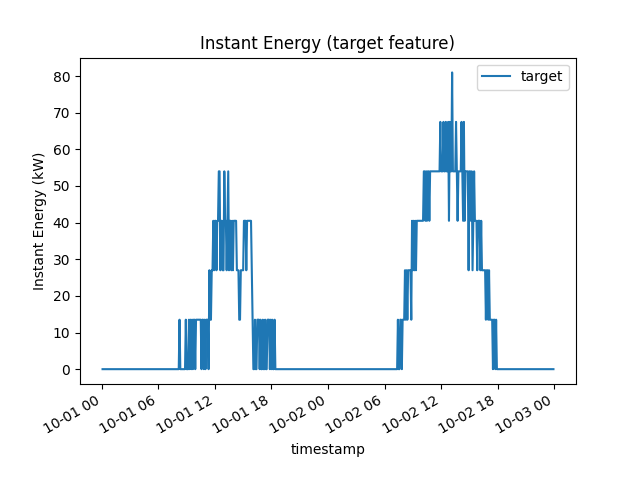
\includegraphics[width=\linewidth, keepaspectratio]{chapters/2_data_preprocessing/imgs/targetfeature.png}
	\caption{Instant Energy (\texttt{target} feature) 2 days plot.}\label{fig:targetfeature}
\end{figure}

\subsection{Re-Sampling}
Finally, after all the operations described above, we obtain a dataset
with samples taken at 5-minute intervals. As we can see from
Figure~\ref{fig:targetfeature}, this data appears to be quite noisy,
which could pose
challenges during the training phase. Moreover, most of the reports
provided by photovoltaic plant operators are at a 15-minute frequency.
To prevent potential issues and align with this standard, we have
written and applied a re-sampling procedure.

%Infine, dopo tutte le operazioni descritte in precedenza, ci troviamo con
%un dataset che ha campioni presi in intervalli di 5 minuti. Come possiamo
%vedere anche dalla Figura \ref{fig:targetfeature} questi dati risultano
%essere abbastanza rumorosi, ciò potrebbe portare a delle difficoltà 
%nella fase di addestramento. In più la maggiorpare dei report che vengono
%forniti dai gestori di impianti fotovoltaici sono ad una frequenza di 15 minuti. Per prevenire eventuali problemi ed adeguarci a questo standard
%abbiamo scritto ed applicato una procedura di Re-Sampling.
%

\begin{algorithm}[H]
	\caption{15 minute Re-Sampling Algorithm.}\label{alg:resampling}
	\begin{algorithmic}
		\Require dataset table
		\Ensure \texttt{dataset} \textbf{is not} empty

		\For{\textbf{each} feature \textbf{in} dataset.features}
		\If{feature \textbf{is} Cumulative}
		\State feature $\gets$ sample \texttt{feature} column using 15 min. sampling rate
		\Else
		\State feature $\gets$ aggregate values every 15 minutes and sum them to form a single value
		\EndIf
		\EndFor
	\end{algorithmic}
\end{algorithm}

\begin{figure}[H]
	\centering
	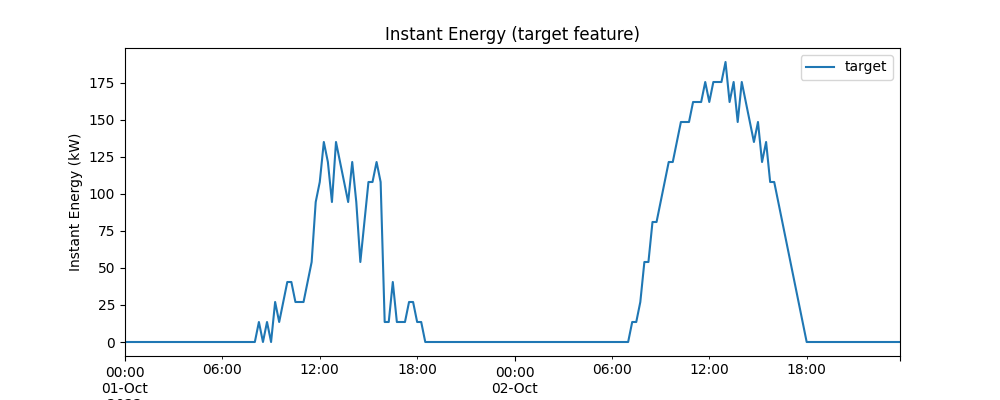
\includegraphics[width=\linewidth, keepaspectratio]{chapters/2_data_preprocessing/imgs/targetfeature15min.png}
	\caption{Instant Energy feature on 15 minute re-sampled dataset.}\label{fig:15min}
\end{figure}


\newpage
%% PPS viene da: https://towardsdatascience.com/rip-correlation-introducing-the-predictive-power-score-3d90808b9598
\section{Feature Selection}\label{sec:featureselection}
After applying all the procedures described in the previous section,
we find ourselves with a dataset composed of 764 columns.
This high number of features would make it nearly impossible to train various models,
both from a purely hardware perspective and due to the excessive information redundancy.
In an attempt to minimize the number of features as much as possible,
we applied and combined the results of two essential tools for feature selection:
the \textit{Correlation Matrix}\cite{corr} and the \textit{Power Predictive Score}\cite{pps}.

%Dopo aver applicato tutte le procedure descritte nella precedente sezione,
%ci ritroviamo con un dataset formato da 764 colonne. Questo elevato
%numero di features renderebbe quasi impossibile l'allenamento dei vari
%modelli, sia dal punto di vista puramente hardware che per l'eccessiva 
%ridondanza delle informazioni. Per cercare di ridurre il più possibile
%il numero di features abbiamo applicato e unito i risultati di due
%strumenti fondamentali per la fearue selection: Correlation Matrix e Power Predictive Score.

\begin{figure}[H]
	\centering
	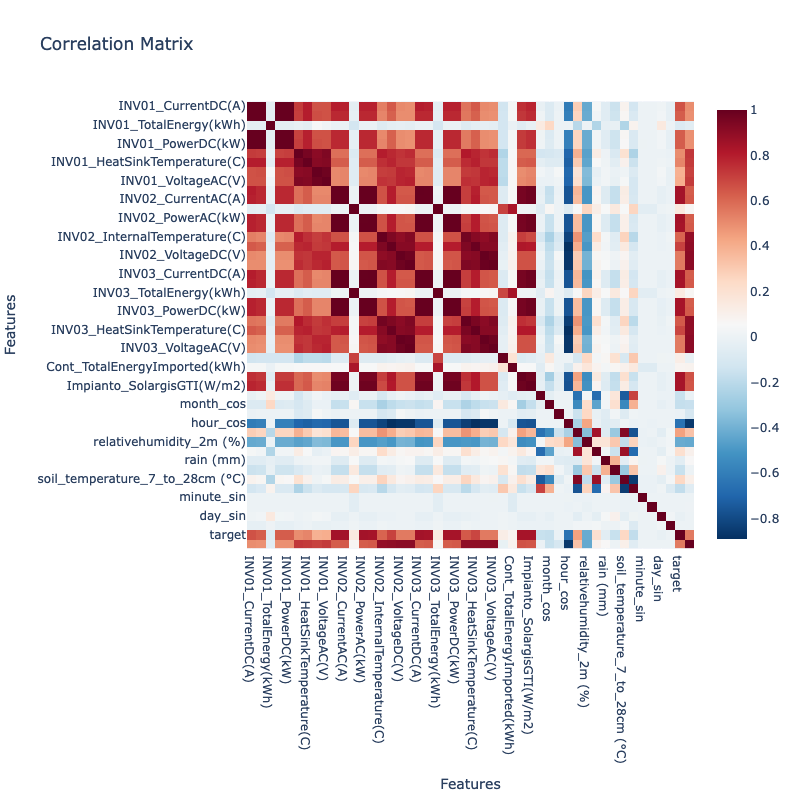
\includegraphics[width=\textwidth, keepaspectratio]{chapters/2_data_preprocessing/imgs/correlationmatrix.png}
	\caption{Correlation Matrix}\label{fig:corrmatrix}
\end{figure}
As we can infer, even with a naive approach, all the information from the various
String Boxes and Junction Boxes is perfectly summarized by the data provided by the
various Inverters (see Section~\ref{sec:pv}); a similar reasoning can be applied to the features
coming from \textit{Other} (those starting with \verb|other_|), as they do not provide any
useful information for energy estimation. Consulting the Correlation Matrix (Figure~\ref{fig:corrmatrix}), we can
see that this naive reasoning is confirmed because the features of the junction boxes
have a high level of correlation with those of the Inverters.
In general, we want to retain features that are minimally correlated with each other
and aim to discard highly correlated ones, keeping only those that are more representative.

%Come possiamo intuire, anche con un approccio naive, tutte  le informazioni delle varie String Box e Junction Box vengono riassunte perfettamente dai dati
%che ci forniscono i vari Inverter (vedi Sezione \ref{sec:pv}); un quasi simile
%ragionamento può essere fatto per le feature che provengono da \textit{Other} (quelle che iniziano con \verb|other_|) dato che non apportano nessuna
%informazione utile alla stima dell'energia.
%Consultando la Correlation Matrix possiamo vedere che questo ragionamento
%naive è confermato, in quanto le feature delle junction box hanno un alto
%tasso di correlazione rispetto a quelle degli Inverter. In generale,
%vogliamo tenere feature che sono poco correlate tra di loro e cercare di 
%scartare quelle molto correlate tenendone solo alcune che sono più 
%rappresentative.
Applying this approach straightforwardly, however, is not the best choice because it
could lead to the loss of important information.
Let's consider an example: let's take into account the features \verb|INV01_Power(kW)|,
\verb|INV02_Power(kW)|, and \verb|INV03_Power(kW)|; by examining the correlation matrix, these
three features are highly correlated, and, therefore, we should retain only one of them.
However, all three are important for predicting our target.
For instance, if Inverter 1 experiences any issues and is not operating at 100\%,
this will impact the total energy production, making all three of these
features indispensable. Therefore, in conjunction with the correlation matrix,
we have utilized the \textit{Power Predictive Score} (PPS): an asymmetric,
data-type-agnostic score that can detect linear or non-linear relationships
between two or more columns\cite{pps}. The score ranges from 0 (no predictive power)
to 1 (perfect predictive power)\cite{pps}.

%Applicare questo approccio in modo straight forward non è però la scelta migliore,
%in quanto potrebbe farci perdere informazioni importanti.
%Facciamo un esempio: prendiamo in considerazione le features \verb|INV01_Power(kW)|, \verb|INV02_Power(kW)| e \verb|INV03_Power(kW)|;
%controllando la matrice di correlazione queste 3 risutano estremamente correlate
%e quindi ne dovremmo tenere soltanto una, ma tutte e 3 risultano importanti
%ai fini della predizione del nostro target: se, per esempio, l'Inverter 1 ha
%avuto qualche problema e non è operativo al 100\% questo si va a riflettere
%sull'energia totale prodotta, rendendo queste feature tutte e 3 indispensabili.
%Abbiamo quindi utilizzato in concomitanza alla matrice di correlazione il \textit{Power Predictive Score} (PPS): an asymmetric, data-type-agnostic
%score that can detect linear or non-linear relationships between two or more columns.
%The score ranges from 0 (no predictive power) to 1 (perfect predictive power).
%
\begin{figure}[H]
	\centering
	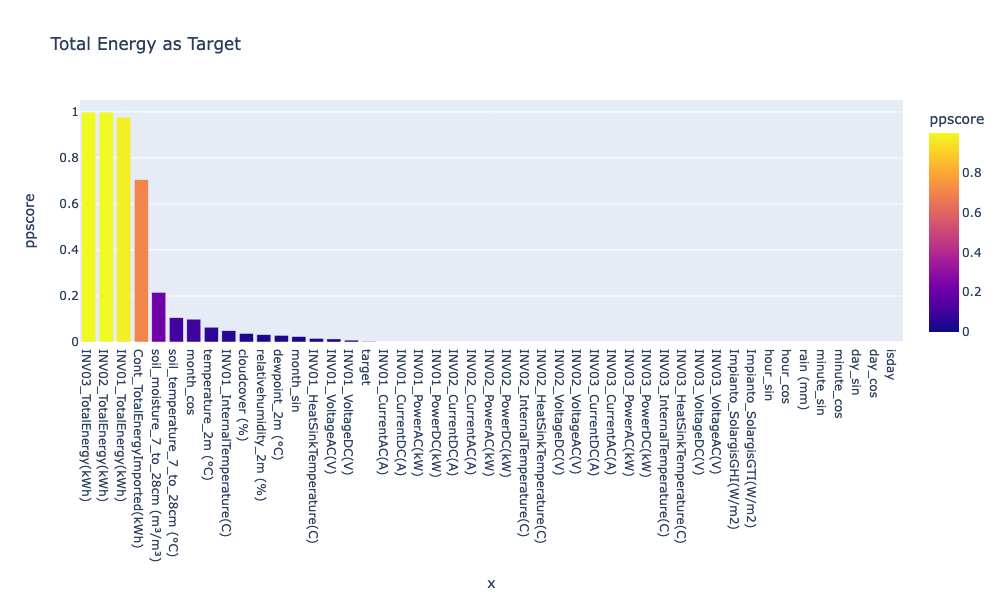
\includegraphics[width=.9\textwidth, keepaspectratio]{chapters/2_data_preprocessing/imgs/ppcontottenergy.png}
	\caption{All features PPS using \texttt{Cont\_TotalEnergy(kWh)} as target.}\label{fig:ppsTotEnergy}
\end{figure}


\begin{figure}[H]
	\centering
	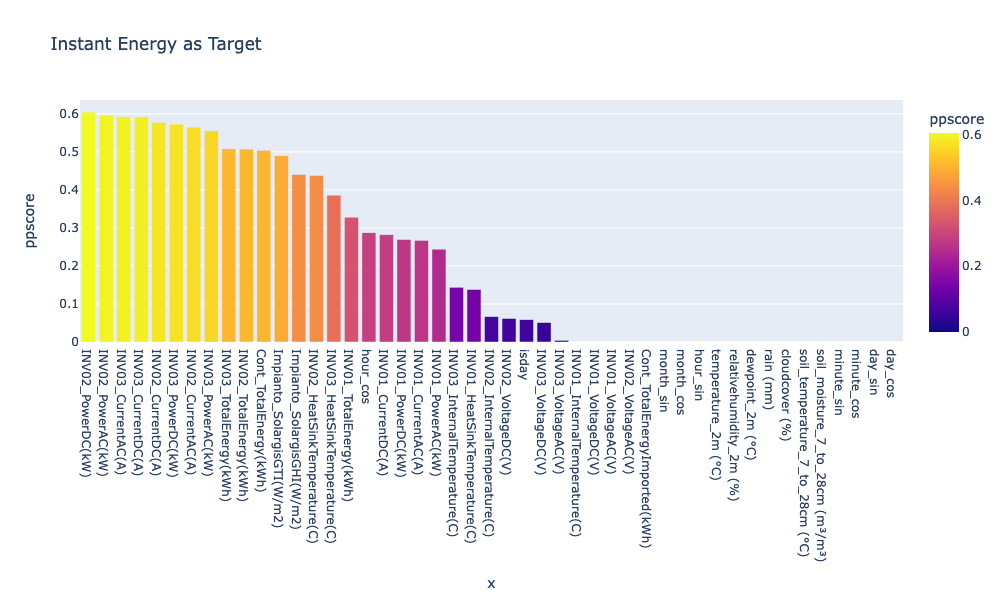
\includegraphics[width=.9\textwidth, keepaspectratio]{chapters/2_data_preprocessing/imgs/pptarget.png}
	\caption{All feature PPS using Instant Energy (\texttt{target}) as Target.}\label{fig:ppstarget}
\end{figure}

As we can see in Figures~\ref{fig:ppsTotEnergy} and \ref{fig:ppstarget}, the features
that perform better in predicting the instantaneous energy production trend are
indeed those of the Inverters, confirming the reasoning described earlier.
Finally, by combining the results obtained from the Correlation Matrix and the
Power Predictive Score, we obtain a final set of 32 features.

%Come possiamo vedere nelle Figure \ref{fig:ppsTotEnergy} e \ref{fig:ppstarget}
%le feature che riescono meglio a predirre l'andamento dell'energia istananea
%prodotta sono proprio quelle degli Inverter, confermando quindi il ragionamento
%descritto prima.
%Infine, combinando i risultati ottenuti dalla Correlation Matrix e dal PPS,
%otteniamo un set finale di 28 features.
%
\begin{table}[H]
	\begin{center}
		\begin{tabular}[t]{l|}
			\verb|INV01_PowerAC(kW)|      \\
			\verb|INV01_PowerDC(kW)|      \\
			\verb|INV02_PowerAC(kW)|      \\
			\verb|INV02_PowerDC(kW)|      \\
			\verb|INV03_PowerAC(kW)|      \\
			\verb|INV03_PowerDC(kW)|      \\
			\verb|INV01_CurrentAC(A)|     \\
			\verb|INV01_CurrentDC(A)|     \\
			\verb|INV02_CurrentAC(A)|     \\
			\verb|INV02_CurrentDC(A)|     \\
			\verb|INV03_CurrentAC(A)|     \\
			\verb|INV03_CurrentDC(A)|     \\
			\verb|INV01_TotalEnergy(kWh)| \\
			\verb|INV02_TotalEnergy(kWh)|
		\end{tabular}
		\begin{tabular}[t]{l|}
			\verb|INV03_TotalEnergy(kWh)|       \\
			\verb|INV01_HeatSinkTemperature(C)| \\
			\verb|INV02_HeatSinkTemperature(C)| \\
			\verb|INV03_HeatSinkTemperature(C)| \\
			\verb|Impianto_SolargisGHI(W/m2)|   \\
			\verb|Impianto_SolargisGTI(W/m2)|   \\
			\verb|rain (mm)|                    \\
			\verb|cloudcover (%)|               \\
			\verb|hour_sin|                     \\
			\verb|hour_cos|                     \\
			\verb|day_sin|                      \\
			\verb|day_cos|                      \\
			\verb|month_sin|                    \\
			\verb|month_cos|
		\end{tabular}
		\begin{tabular}[t]{l}
			\verb|min_sin| \\
			\verb|min_cos| \\
			\verb|target|
		\end{tabular}
	\end{center}
	\caption{All feature selected after this phase.}\label{tab:featselected}
\end{table}


%\begin{figure}[H]
%    \centering
%        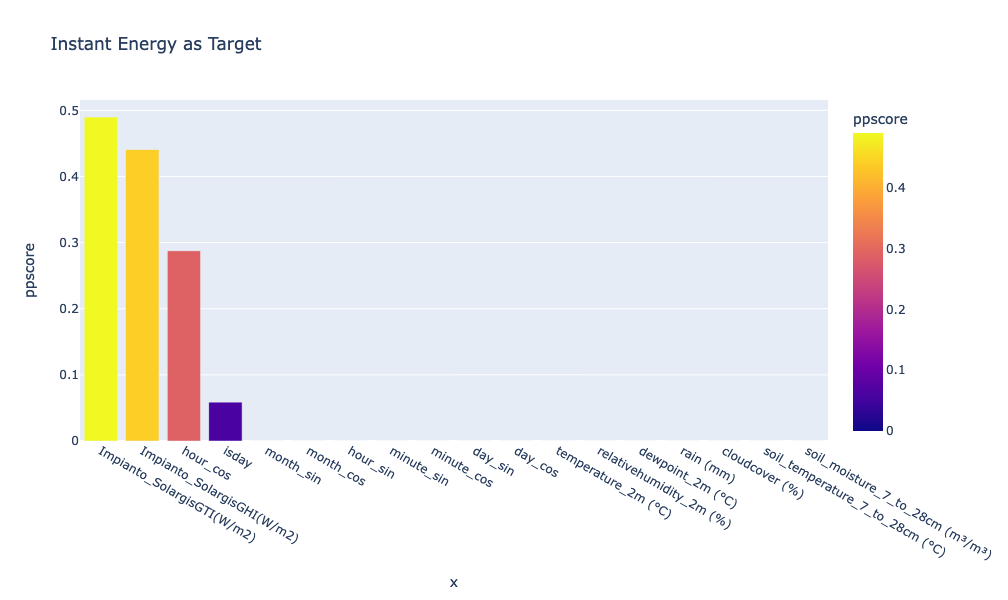
\includegraphics[width=\textwidth, keepaspectratio]{chapters/2_data_preprocessing/imgs/ppbucotarget.png}
%    \caption{Only Wather features PPS using Instant Energy (\texttt{target}) as Target.}
%    \label{fig:ppssolargis}
%\end{figure}
\section{Dataset Splitting}\label{sec:datasetsplitting}
After completing the Feature Selection phase (Section~\ref{sec:featureselection}),
we decided to divide the obtained
dataset into three different sets:

%Completata anche la fase di Feature Selection (Sezione
%\ref{sec:featureselection}) abbiamo deciso di suddividere il dataset
%ottenuto in 3 differenti set:

\begin{itemize}
	\item \textit{Training}: It covers the period from 01-06-2022 to
	      28-02-2023. This set will be used during the training phase
	      to allow the model to learn the plant's performance and how
	      to predict energy trends during various gaps.
	      It starts in June because there are some issues with the
	      Inverter 1's features before that.

	      % comprende il periodo che va dal 01-06-2022
	      %     al 28-02-2023. Questo set sarà utilizzato durante la fase di Training
	      %     per permettere al modello di apprendere l'andamento dell'impianto e 
	      %     come riuscire a prevedere l'andamento dell'energia durante i vari buchi. Parte da giugno perchè prima ci sono alcuni problemi con le feature dell'Inverter 1.
	\item \textit{Validation}: It spans from 01-03-2023 to 31-03-2023.
	      It will be used in the training phase to assess the presence
	      of overfitting or if this phase might have failed.

	      % va dal 01-03-2023 al 31-03-2023. Verrà utilizzato nella fase di training per capire se c'è presenza di overfitting o se questa fase potrebbe aver fallito.
	\item \textit{Test}: It starts on 01-04-2023 and continues
	      until 30-04-2023. This set will be used in the Evaluation phase
	      to estimate the model's performance on a data period it has
	      never seen before.

	      % parte dal 01-04-2023 fino ad arrivare al 30-04-2023. Questo set sarà utilizzato nella fase di Evaluation per
	      % poter stimare le performance del modello su un periodo di dati che non ha mai visto prima.
\end{itemize}

\begin{table}[H]
	\begin{center}
		\begin{tabular}[c]{l|l|l|l}
			%\cline{2-4}
			\multicolumn{1}{c|}{}               &
			\multicolumn{1}{c|}{\textbf{Start}} &
			\multicolumn{1}{c|}{\textbf{End}}   &
			\multicolumn{1}{c}{\textbf{Rows}}                                     \\
			\hline

			\textbf{Training}                   & 01-06-2022 & 28-02-2023 & 24864 \\
			\textbf{Validation}                 & 01-03-2023 & 31-03-2023 & 2880  \\
			\textbf{Testing}                    & 01-04-2023 & 30-04-2023 & 2880
		\end{tabular}
	\end{center}
	\caption{Summary table of how the dataset was divided.}\label{tab:dfsplit}
\end{table}
